Multiple choice section. All points are for choosing the correct answer. No justification is needed.
\begin{questions} 

\question[3] %Ang Complex number

Solve the following quadratic equation:\\
\[x^2+9=0\] [Select \textbf{ONE}]
\begin{checkboxes}
    \choice $x=-3$
    \choice $x=3$
    \choice $x=3$ or $x=-3$
    \choice $x=3i$ or $x=-3i$
    \choice The equation has no solution.
\end{checkboxes}


\question[3] Select the equation of the line through $(-2 , 3)$ \textbf{parallel} to the line $y=-2x+1$. [Select \textbf{ONE}]
\begin{choices}
   \choice \chooseone $y + 3=-2(x-2)$
   \choice \chooseone $y - 3=-2(x+2)$
   \choice \chooseone $y + 3=\frac{1}{2}(x-2)$
   \choice \chooseone $y - 3=\frac{1}{2}(x+2)$
   \choice \chooseone None of the above.
\end{choices}
% Question 3. It says select multiple, but in fact only one solution is correct.
\question[3] Select all real solutions to the equation $\sqrt{7-2x}+1=2x$. [Select \textbf{One or more}]
    \begin{multicols}{2}
    %\checkboxchar{\Large$\Box$}
    \checkboxchar{\Large$\Box$}\begin{checkboxes}
    
    \choice \hspace{-3em} A.\hspace{1.2em} $x=-1$
        \choice \hspace{-3em} B.\hspace{1.2em} $x=1$
    
        \choice \hspace{-3em} C. \hspace{1.2em}$x=\frac{3}{2}$
    
        \choice \hspace{-3em} D.\hspace{1.2em} $x=-\frac{3}{2}$
        
        \end{checkboxes}
    \end{multicols}

\question[3] Select the function graphed below. [Select \textbf{ONE}]

\begin{multicols}{2}
    

    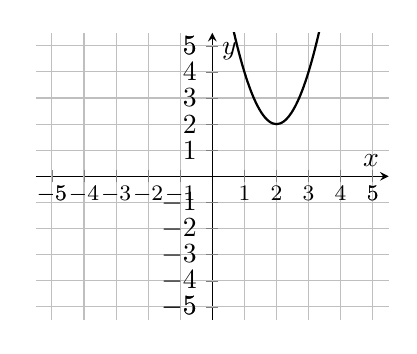
\begin{tikzpicture}
\begin{axis}[
   grid = major,
   extra x ticks={-6,-5,-4,-3,-2,-1,1,2,3,4,5,6},
   extra y ticks={-6,-5,-4,-3,-2,-1,1,2,3,4,5,6},
   %ytick= false,
   %xminorgrids=true,
   width=.5\textwidth,
   %clip = true,
   %clip mode=individual,
   %restrict y to domain=-12:12,
   axis x line = middle,
   axis y line = middle,
   %     yticklabel style = {font=\footnotesize,xshift=0.5ex},
        xticklabel style = {font=\footnotesize,yshift=0.5ex},
   xlabel={$x$},
   %xlabel style={at=(current axis.right of origin)},
   ylabel={$y$},
   %ylabel style={at=(current axis.above origin)},
   %domain = -5:5,
   xmin = -5,
   xmax = 5,
   enlarge y limits={rel=0.05},
   enlarge x limits={rel=0.05},
   ymin = -5,
   ymax = 5,
 ]
\addplot[smooth, thick, domain = 0:4,samples=35
	] { 2*(x-2)^2+2};
% \addplot[smooth, thick, domain = 1.15:6.5,
%	] { (3*x^2+5*x-2)/(x-1)};
\end{axis}
\end{tikzpicture}
\begin{checkboxes}
    \choice \hspace{-3em} A. \hspace{1.2em} $f(x)=-2(x+2)^2-2$
    \choice \hspace{-3em} B. \hspace{1.2em} $f(x)=2(x+2)^2+2$
    \choice \hspace{-3em} C. \hspace{1.2em} $f(x)=2(x-2)^2-2$
    \choice \hspace{-3em} D. \hspace{1.2em} $f(x)=2(x-2)^2+2$
    \choice \hspace{-3em} E. \hspace{1.2em} None of the above.
\end{checkboxes}
\end{multicols}

\newpage
\question[3] Determine where the function is increasing. [Select \textbf{ONE}]

\begin{multicols}{2}
    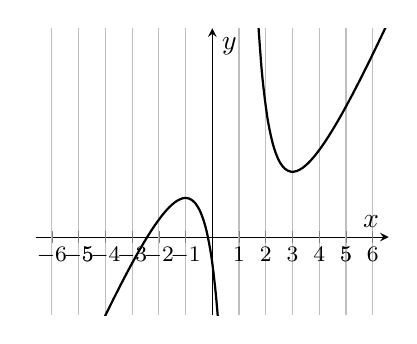
\begin{tikzpicture}
\begin{axis}[
   grid = major,
   extra x ticks={-6,-5,-4,-3,-2,-1,1,2,3,4,5,6},
   %extra y ticks={-6,-5,-4,-3,-2,-1,1,2,3,4,5,6},
   ytick= false,
   %xminorgrids=true,
   width=.5\textwidth,
   %clip = true,
   %clip mode=individual,
   %restrict y to domain=-12:12,
   axis x line = middle,
   axis y line = middle,
   %     yticklabel style = {font=\footnotesize,xshift=0.5ex},
        xticklabel style = {font=\footnotesize,yshift=0.5ex},
   xlabel={$x$},
   %xlabel style={at=(current axis.right of origin)},
   ylabel={$y$},
   %ylabel style={at=(current axis.above origin)},
   %domain = -5:5,
   xmin = -6,
   xmax = 6,
   enlarge y limits={rel=0.05},
   enlarge x limits={rel=0.05},
   ymin = -5,
   ymax = 15,
 ]
\addplot[smooth, thick, domain = -6.5:0.87,samples=35
	] { 5*(x^2+3*x)/(x-1)-2};
 \addplot[smooth, thick, domain = 1.15:6.5,
	] { 5*(x^2+3*x)/(x-1)-40};
\end{axis}
\end{tikzpicture}

%\begin{multicols}{2}
    
\begin{checkboxes}
    \choice \hspace{-3em} A. \hspace{1.2em} $(-\infty,\infty)$
    \choice \hspace{-3em} B. \hspace{1.2em} $(-\infty,-1)\cup (3,\infty)$
    \choice \hspace{-3em} C. \hspace{1.2em} $(3,\infty)$
    \choice \hspace{-3em} D. \hspace{1.2em} $(-\infty,1)\cup (1,\infty)$
    \choice \hspace{-3em} E. \hspace{1.2em} None of the above.
\end{checkboxes}
\end{multicols}

\question[3] Select the graph of the function below. [Select \textbf{ONE}]
    \vspace{-0.2cm}
    \begin{equation*}
        f(x)=(x+2)^2(x+1)(x-1).
    \end{equation*}
    \vspace{.2cm}


    
    \begin{choices}
      \begin{multicols}{2}
        	
        	
    
        		\choice \chooseone\vspace{-.7cm}
        		
        	\hspace{.1cm}	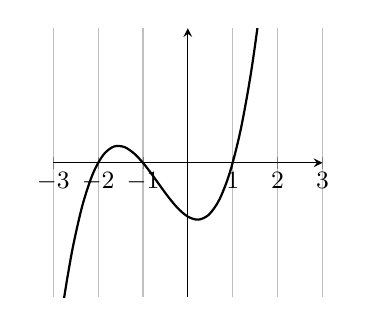
\begin{tikzpicture}%[domain=-4:4]
        			\begin{axis}[
        				grid=major,
        				axis x line = middle,
        				axis y line = middle,
        				%yticklabel style = {font=\tiny,xshift=0.5ex},
        				xticklabel style = {font=\small,yshift=0.5ex},
        				%scale only axis=true,
        				width=5 cm,
        				height=5 cm,
        				xtick={-3,-2,-1,0,1,2,3},%{-2,-1,0,1,2},
        				ytick=false,%{-2,-1,0,1,2,3,4},
        				xmin=-3,
        				xmax=3,
        				ymin=-5,
        				ymax=5,
        				]
        				%\draw[very thin,color=gray] (-2.9,-2.1) grid (2.9,2.9);
        				\addplot[smooth, thick, domain = -4:4,samples=35] { (x+2)*(x+1)*(x-1)};
        				%\addplot[smooth, thick, domain = 0:3,samples=35] { -x};
        			\end{axis}
        		\end{tikzpicture}
        		
        \choice \chooseone\vspace{-.7cm}
        		
        \hspace{.1cm}	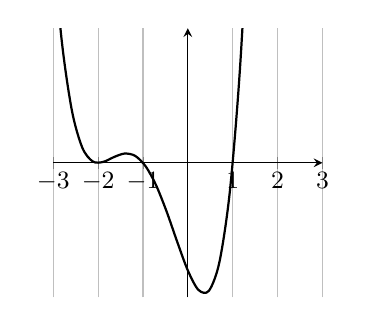
\begin{tikzpicture}%[domain=-4:4]
    	\begin{axis}[
    		grid=major,
    		axis x line = middle,
    		axis y line = middle,
    		%yticklabel style = {font=\tiny,xshift=0.5ex},
    		xticklabel style = {font=\small,yshift=0.5ex},
    		%scale only axis=true,
    		width=5 cm,
    		height=5 cm,
    		xtick={-3,-2,-1,0,1,2,3},%{-2,-1,0,1,2},
    		ytick=false,%{-2,-1,0,1,2,3,4},
    		xmin=-3,
    		xmax=3,
    		ymin=-5,
    		ymax=5,
    		]
    		%\draw[very thin,color=gray] (-2.9,-2.1) grid (2.9,2.9);
    		\addplot[smooth, thick, domain = -4:4,samples=35] { (x+2)^2*(x+1)*(x-1)};
    		%\addplot[smooth, thick, domain = 0:3,samples=35] { -x};
    	\end{axis}
    \end{tikzpicture}
        	\choice \chooseone\vspace{-.7cm}
        		
        	\hspace{.1cm}	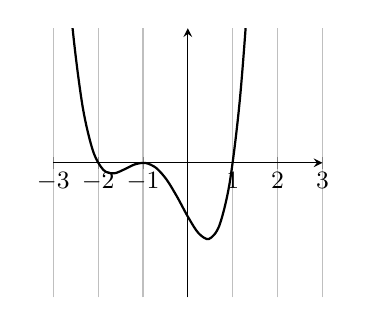
\begin{tikzpicture}%[domain=-4:4]
    	\begin{axis}[
    		grid=major,
    		axis x line = middle,
    		axis y line = middle,
    		%yticklabel style = {font=\tiny,xshift=0.5ex},
    		xticklabel style = {font=\small,yshift=0.5ex},
    		%scale only axis=true,
    		width=5 cm,
    		height=5 cm,
    		xtick={-3,-2,-1,0,1,2,3},%{-2,-1,0,1,2},
    		ytick=false,%{-2,-1,0,1,2,3,4},
    		xmin=-3,
    		xmax=3,
    		ymin=-5,
    		ymax=5,
    		]
    		%\draw[very thin,color=gray] (-2.9,-2.1) grid (2.9,2.9);
    		\addplot[smooth, thick, domain = -4:4,samples=35] { (x+2)*(x+1)^2*(x-1)};
    		%\addplot[smooth, thick, domain = 0:3,samples=35] { -x};
    	\end{axis}
    \end{tikzpicture}
        	\choice \chooseone\vspace{-.7cm}
        		
        	\hspace{.1cm}	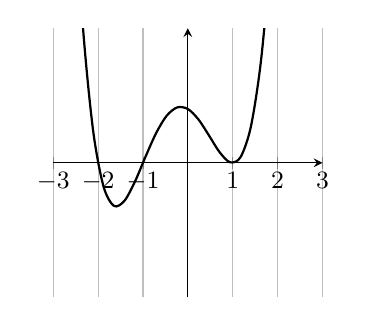
\begin{tikzpicture}%[domain=-4:4]
    	\begin{axis}[
    		grid=major,
    		axis x line = middle,
    		axis y line = middle,
    		%yticklabel style = {font=\tiny,xshift=0.5ex},
    		xticklabel style = {font=\small,yshift=0.5ex},
    		%scale only axis=true,
    		width=5 cm,
    		height=5 cm,
    		xtick={-3,-2,-1,0,1,2,3},%{-2,-1,0,1,2},
    		ytick=false,%{-2,-1,0,1,2,3,4},
    		xmin=-3,
    		xmax=3,
    		ymin=-5,
    		ymax=5,
    		]
    		%\draw[very thin,color=gray] (-2.9,-2.1) grid (2.9,2.9);
    		\addplot[smooth, thick, domain = -4:4,samples=35] { (x+2)*(x+1)*(x-1)^2};
    		%\addplot[smooth, thick, domain = 0:3,samples=35] { -x};
    	\end{axis}
    \end{tikzpicture}
    \end{multicols}
    
      \centering \choice \chooseone None of the above.
    \end{choices}

\newpage
\hspace{-.5in}Free answer section. Work must be shown to get credit for any answer. Partial credit may be given even for incorrect final answers, so show your work.

% \question question
% \begin{parts}
% 	\part[5] part a
% 	%\vspace{5cm}
%     \vfill
% 	\part[6] part b
% 	%\vspace{6cm}
%     \vfill
% \end{parts}

% \newpage

\question[6] Solve the following inequality and write your answers using interval notation.
% \begin{parts}
% 	\part[5]  
 %    $x^2 -8x < -15$.
	% %\vspace{5cm}
 %    \vfill
%	\part[5] 
    \[|2x+3|+1 \leq 6\].
	%\vspace{6cm}
    \vfill\vfill

    $ \mbox{Solution: } \Scale[1.5]{\boxed{ \phantom{\dfrac{a}{b}} \hspace{8cm} }}$
% \end{parts}
\question[4] Expand the logs with no interior multiplications or divisions and simplified powers as much as the rules allow.
    \[ \ln \frac{y^2}{\sqrt{2^x (z+x)^3}} \]
     
    \vfill
$
            \ln \frac{y^2}{\sqrt{2^x (z+x)^3}}= \Scale[1.5]{\boxed{ \phantom{\dfrac{a}{b}} \hspace{8cm} }}
            $
\newpage

%Logan wrote this for 2.7-2.8. It might be too hard.
\question%[10]
    Consider the function $f(x)=\dfrac{2x-5}{x+4}$. (Graph shown below.)

           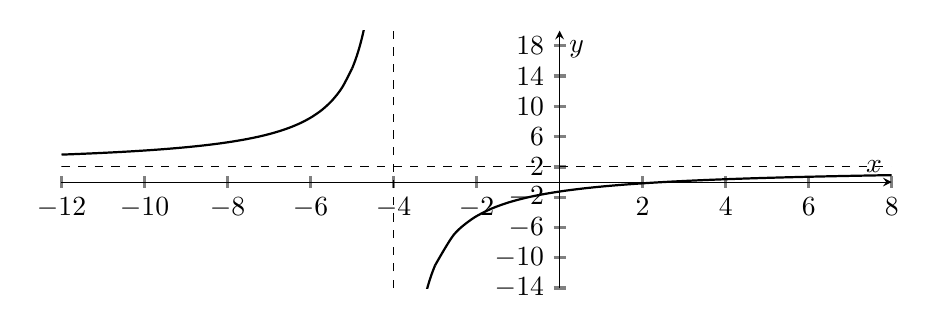
\begin{tikzpicture}
\begin{axis}[
  width= \textwidth,
  height= .4\textwidth,
  axis lines=middle,
  %grid=major,
  xmin=-12,
  xmax=8,
  ymin=-14,
  ymax=20,
  xlabel=$x$,
  ylabel=$y$,
  xtick={-12,-10,...,10},
  ytick={-14,-10,...,20},
  tick style={very thick},
  % legend style={
  % at={(rel axis cs:0,1)},
  % anchor=north west,draw=none,inner sep=0pt,fill=gray!10}
]
\addplot[smooth, thick, domain = -12:-5,samples=30] { (2*x-5)/(x+4)};
\addplot[smooth, thick, domain = -5:-4.15,samples=30] { (2*x-5)/(x+4)};
\addplot[smooth, thick, domain = -3.85:-3,samples=30] { (2*x-5)/(x+4)};
\addplot[smooth, thick, domain = -3:10,samples=30] { (2*x-5)/(x+4)};
\addplot[dashed, domain =-12:8, samples = 2]{2};
\draw[dashed](axis cs:-4, -14) -- (axis cs:-4, 20);
\end{axis}
\end{tikzpicture}
    \begin{parts}
        \part[2] What is the domain and range of $f(x)$? (Write in interval notation.)
        \begin{multicols}{2}
            $
                \mbox{Domain: } \Scale[1.7]{\boxed{ \phantom{\dfrac{a}{b}} \hspace{3cm} }}
            $
            \\
            $
                \mbox{Range: } \Scale[1.7]{\boxed{ \phantom{\dfrac{a}{b}} \hspace{3cm} }}
            $
            \end{multicols}
%\vfill
        \part[4] What are the domain and range of $f^{-1}(x)$? (Write in interval notation.)
        \begin{multicols}{2}
            $
                \mbox{Domain: } \Scale[1.7]{\boxed{ \phantom{\dfrac{a}{b}} \hspace{3cm} }}
            $
            \\
            $
                \mbox{Range: } \Scale[1.7]{\boxed{ \phantom{\dfrac{a}{b}} \hspace{3cm} }}
            $
            \end{multicols}
        \part[5] What is $f^{-1}(x)$?
\vfill
$
                f^{-1}(x) = \Scale[1.5]{\boxed{ \phantom{\dfrac{a}{b}} \hspace{5cm} }}
            $
    \end{parts}

\newpage


%Jingyi Section3.3
\question  %\todo[inline]{Can we rewrite this as a slant asymptote question?}
 %   Perform the polynomial division below, and identify the quotient $Q(x)$ and remainder $R(x)$.
  Consider the rational function     
    \begin{equation*}
       f(x)= \dfrac{x^3-13 x^2+40 x+18}{ x^2-7x}
    \end{equation*}

 \begin{parts}
     
\part[8] Perform the division and write $f(x)$ as $f(x)= Q(x)+\dfrac{R(x)}{D(x)}$
    
\vfill\vfill\vfill\vfill\vfill
$
                f(x) = \Scale[2]{\boxed{ \phantom{\dfrac{a}{b}} \hspace{6cm} }}
            $
\part[2] Does $f(x)$ have a slant asymptote? If so what is it? If not write ``DNE".

$
              \mbox{slant asymptote: }   \Scale[1.7]{\boxed{ \phantom{\dfrac{a}{b}} \hspace{4cm} }}
            $
 \end{parts}
\newpage

\question  
    A basketball player throws a half court shot. Let $t$ denote the time taken (in seconds) after the ball was released. At $t=0$, they release the ball at the height of 10ft. At $t=2$, the ball reaches the basket, which is also 10ft high. The height of the ball $h$ (in ft) can be modeled by the following equation: \[h(t)=a(t-1)^2+k.\]
\begin{parts}
    

\part[4]    It is given that the maximum height of the ball is 15ft. Based on the information above, find the values of $a$ and $k$ in the equation of $h(t)$.
   
\vfill
$a$ = \Scale[1.5]{\boxed{ \phantom{\dfrac{a}{b}} \hspace{1cm} }}, $k$ = \Scale[1.5]{\boxed{ \phantom{\dfrac{a}{b}} \hspace{1cm} }}
\part[2] What time $t$ will the ball reach its maximum height?\\
$
                t = \Scale[1.5]{\boxed{ \phantom{\dfrac{a}{b}} \hspace{2cm} }}
            $

\end{parts} 

\question[6] Find all roots of the polynomial: $x^4 + x^2 - 12$. (Roots may be real, complex or a combination.)

\vfill

$
            \mbox{Roots: } \Scale[1.5]{\boxed{ \phantom{\dfrac{a}{b}} \hspace{8cm} }}
            $

\newpage

%Section 3.7, Logan's Problem. Easier version: solve the inequality f(x)\ge g(x). I want the nonstrict inequality here b/c it results in intervals which are neither open nor closed.
\question[8] Find all values of $x$ that satisfy the following inequality:

\[\displaystyle \frac{x}{x-11}\displaystyle \ge \frac{100}{x^2-11x}.\] Write your answer in interval notation. %(You must show work.)

\vfill
Interval: $\Scale[1.7]{\boxed{ \phantom{\dfrac{a}{b}} \hspace{6cm} }}$



% \newpage


%Yuchen Sec. 4.3-4.4

\question[7] Solve the following equation. If no solution exists, write ``DNE''.
\[\log_2 (x-1)+\log_2 (x+6)=3\]

    % \todo[inline]{or do we want to find the negative?}
    % \[\log_2 (1-x)+\log_2 (-x-6)=3\]
	%\vspace{5cm}
    \vfill

	%\vspace{6cm}
 %   \vfill
$
                x = \Scale[1.5]{\boxed{ \phantom{\dfrac{a}{b}} \hspace{3cm} }}
            $

\newpage
%Yewei Sec. 5.1
\question[8]
For the following system of linear equations, determine whether or not the system has any solutions. If the system has a solution, state it as an ordered pair $(x,y)$; if the systems has infinitely many solutions, write your solutions as an ordered pair in terms of the variable $x$ only.
$$\begin{cases}
3 x  +  4 y & = 1 \\
- x  +  2 y & = 8
\end{cases}$$
% Solution is $(x,y)=(3,-2)$

\vfill

$
                (x,y) = \Scale[1.5]{\boxed{ \phantom{\dfrac{a}{b}} \hspace{3cm} }}
            $
\newpage 



\newpage
\question Consider the function $$f(x) = \frac{(2x+1)(x-2)}{3x(x-2)(x+3)^2} $$%= \frac{2x^2-3x-2}{3x^4-9x^2-6x}$$

\begin{parts}
        \part[2] Find the zero(s) of $f(x)$. If none exist, write ``DNE". 
        
        \vfill
        $
                \mbox{zero(s)} = \Scale[1.5]{\boxed{ \phantom{\dfrac{a}{b}} \hspace{3cm} }}
            $
        \part[2] Find the vertical asymptote(s) of $f(x)$. If none exist, write ``DNE".
        \vfill
        
        $
                \mbox{Vertical Asymptotes} = \Scale[1.5]{\boxed{ \phantom{\dfrac{a}{b}} \hspace{3cm} }}
            $
        \part[2] What can we say about the graph of f(x)? [Select \textbf{ONE}]     
            \begin{choices}
               \choice \chooseone $f(x)$ has a horizontal asymptote at $y = 0$
               \choice \chooseone $f(x)$ has a horizontal asymptote at $y = \dfrac{2}{3}$ %Or $y\neq 0$ not sure which choice is better
               \choice \chooseone $f(x)$ has a slant asymptote.
               \choice \chooseone None of the above.
            \end{choices}
        %\vspace{1cm}
        % \part[4] Express, in interval notation, where $f(x)>0$.
        % \vspace{5cm}
        % \newpage

        \part[4] Sketch this function on the axis below. Make sure to label \underline{zeroes}, \underline{asymptotes} and \underline{holes} on your sketch.

        
        \begin{tikzpicture}
\begin{axis}[
  width= \textwidth,
  height= .8\textwidth,
  axis lines=middle,
  %grid=major,
  xmin=-4.5,
  xmax=4.5,
  ymin=-4,
  ymax=4,
  xlabel=$x$,
  ylabel=$y$,
  xtick={-4,-3,...,4},
  ytick=false,%{-4,-3,...,4},
  tick style={very thick},
  legend style={
  at={(rel axis cs:0,1)},
  anchor=north west,draw=none,inner sep=0pt,fill=gray!10}
]
\end{axis}
\end{tikzpicture}
    \end{parts}

\question %In a different petri dish a
A group of scientists are trying to develop a treatment to stop the planarians from growing. 
\begin{parts}
    \part[4]
Sample A starts with 1000 planarians, and 2 hours later there are 200 planarians. 
 Find a function $P(t)=P_0e^{rt}$ that models the population of the planarians after $t$ hours. (Leave the value for $r$ in terms of a $\log$) 
   \vfill\vfill
    \begin{align*}
                \Scale[1.7]{\boxed{P(t) =\phantom{\frac{1}{2}} \hspace{4cm} }}
            \end{align*} %thank you thank you thank you
  
\part[2] %Upon more studies 
The scientists find that the number of planarians in sample B $t$ hours after treatment is best modeled by the function \[P(t) = 800 e^{0.5\ln(1/3)t}.\] Is this function increasing or decreasing? [Select \textbf{ONE}]
\begin{choices}
   \choice \chooseone Increasing
   \choice \chooseone Decreasing
\end{choices}
   Explain how you know based on this model.
%\vspace{3cm}
    % \part[5] Using this new model when will there be $100$ planarians in the petri dish? (Leave your answer in terms of a $\log$)
\vfill
\end{parts}
\end{questions}